\documentclass[12pt]{article}
\usepackage[margin=1.5in]{geometry}
\usepackage{graphicx}
\usepackage{titlesec}
\setlength{\parindent}{0em}
\setlength{\parskip}{0.5em}
\usepackage{enumitem}
\usepackage{mdwlist}
\usepackage{color}
\usepackage{sectsty}
\usepackage{amsmath}

\definecolor{ao}{rgb}{0.0, 0.5, 0.0}
\sectionfont{\color{ao}}

\title{\vspace{-0.5in}Wave Stuff}
\author{}
\date{}

\begin{document}
\maketitle

\vspace{-1in}

\section*{A}

\subsection*{acoustic waves (aka sound waves)}
\begin{itemize*}
    \item Longitudinal
    \item Isotropic
    \item Compressible (propagate by means of adiabatic
        compression and decompression)
    \item travel at sound speed (determined by the medium in which
        they were \emph{created}, and maintain this speed even if they
        travel into medium with a different characteristic sound speed).
    \item Important quantities:
        \begin{itemize*}
            \item sound pressure
            \item particle velocity
            \item particle displacement
            \item sound intensity
        \end{itemize*}
    \item exist because of a pressure restoring force: local compression
        (or rarefaction) sets up a \emph{pressure gradient} in opposition
        to the motion
    \item carry energy away from source
    \item large enough amplitude $\rightarrow$ shock wave,
        but usually small; ambient gas slightly disturbed
    \item exist in medium with low or non-existent magnetic field
    \item isotropic \- propagate equally in all directions. The phase
        and group velocities are both equal to the sound speed (hence, the
        part where acoustic waves are sound waves).
\end{itemize*}

\subsection*{Alfv\'en waves}
Alfv\'en waves are a type of MHD wave in which ions oscillate in response to a 
restoring force provided by an effective tension on the magentic field lines.
Low frequency (compared to the ion cyclotron frequency) traveling
oscillation of the ion and the magnetic field. The ion mass
density provides the inertia and the magnetic field line
tension provides the restoring force.
They propagate in the direction of the magnetic field, although waves exist
at \emph{oblique} incidence and smoothly change into the \emph{magnetoacoustic}
wave when the propagation is \emph{perpendicular} to the magnetic field.
The motion of the ions and the perturbation of the magnetic
field are in the same direction and transverse to the direction of
propagation. The wave is dispersionless.

Locally supported, phase and group velocities with magnitude equal to
local Alfv\'en spped, directed along the magnetic field.
Alfv\'en waves are easily excited by various dynamical perturbations of
magnetic field lines, and are
weakily dissipative (can propagate long distances, deposit energy
and momentum far from source).

Properties:
\begin{itemize*}
    \item m$=$0 (Axisymmetric, or azimuthally symmetric)
    \item transverse (shear) perturbations (perpendicular to $\vec{F}_{res}$);
        plasma has characteristic elasticity.
    \item parallel to $\vec{B}$ (the \emph{group} velocity  is strictly along
        $\vec{B}$, but the \emph{phase} velocity doesn't have to be. The
        energy also propagates along the field lines, probably because the
        wave envelope is what carries all the information).
    \item (only) driving force: magnetic tension, which ``snaps'' the field back
        into a straight line, producing an Alfv\'en wave.
    \item Purely magnetic and incompressible in nature (in untwisted straight
        cylinder$\ldots$ twist may cause some compression).
    \item Displacement of plasma together with magnetic field frozen
        into it.
    \item velocity: $v_{A} = \frac{B}{\mu_{o}\rho}$;
        $\sim$ 1000 km s$^{-1}$ in the corona.
\end{itemize*}
How to observe:
\begin{itemize*}
    \item Only get Doppler shifts from \emph{long}-period waves
        ($>$ a few minutes).
    \item Measure additional (i.e.\ non-thermal) broadening
        of coronal emission lines; indirect way to observe short-period waves.
    \item Spatial variation in Doppler shift for long periods.
        Gyrosynchrotron emission in radio regime.
    \item $V_A$: temporal resolution?
\end{itemize*}
Effects of twisting (or \emph{torsion}):
\begin{itemize*}
    \item Coupling of various MHD modes
\end{itemize*}

(From \emph{Priest}): Types of Alfv\'en waves:
\begin{itemize*}
    \item Shear or Torsional: No accompanying pressure or
        density changes (plasma).
    \item Compressional or Fast-Mode: Becomes a fast
        magnetoacoutsic or fast-mode wave when pressure gradients
        are included (Note: these are often the preferred names,
        even when the pressure gradient is unimportant, so as to
        avoid confusion with shear Alfv\'en waves).
\end{itemize*}

\section*{B}

\subsection*{ballooning modes}
\begin{itemize*}
    \item m $>$ 1

    \item Role not established yet
\end{itemize*}

\subsection*{Bessel's equations}

(From Boas p. 587): Bessel functions are damped sines and cosines.
Solutions of differential equations can be represented by power series.
Graphs, formulas; electricty, heat, hydrodynamics, elasticity, wave motion,
quantum$\ldots$, cylindrical symmetry$\ldots$

Bessel's differential equation:
$$ x^2\frac{d^y}{dx2} + x\frac{dy}{dx} + (x^2-p^2)y = 0 $$
where $p$ is the \emph{order} of the Bessel function $y$ and is a constant, and
$y$ is the solution.
$a$ = integer $\rightarrow$ cylindrical,
$a$ = half-integer $\rightarrow$ spherical.
$$ x^2y'' + xy' + (x^2-p^2)y = 0  $$
$$ x(xy') + (x^2-p^2)y' = 0  $$

\subsection*{body modes}

\section*{C}

\subsection*{coronal loops}
\begin{itemize*}
    \item Main observational feature of the magnetic structure in the
        upper solar atmosphere.
\end{itemize*}

\subsection*{coronal seismology}


\subsection*{cusp speed}
See \emph{tube speed}

\section*{D}

\subsection*{dispersion}
Dispersion is when the distinct phase velocities of the components of the
envelope cause the wave packet to ``spread out'' over time.
The components of the wave packet (or envelope) move apart to the degree
where they no longer combine to complete the envelope.

Causes different components of the wave to have different phase velocities.

Different kinds of dispersion:
\begin{itemize*}
    \item Normal dispersion: strictly increasing Re $\epsilon(\omega)$ with
        increasing $\omega$.
    \item Anomalous dispersion: decreasing Re $\epsilon(\omega)$ with
        increasing $\omega$.
    \item Resonant absorption: occurs in regions where Im $\epsilon(\omega)$
        is large.
\end{itemize*}

\begin{figure}[h]
    \centering
    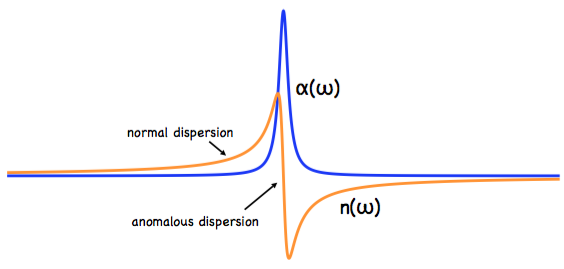
\includegraphics[width=5in]{disp.png}
\end{figure}

No dispersion: $v_{ph} = v_{gr}$; dispersion: $v_{ph} \neq v_{gr}$.
A medium that is free from dispersion has index of refraction that is constant
as a function of frequency, so all wavelengths are similarly affected.
Permittivity and permeability are functions of frequency.
Non-dispersive waves have phase speed ($v_{ph}$, speed that wave actually travels
through medium?) independent of wavenumber, $k$.
All waves of \emph{any} $k$ propagate at the same speed.
Uniform dissipation, resonant mode conversion, physical mechanisms vs. ?

Dispersion \emph{relation}:
\begin{itemize*}
    \item Relates the wavelength (or wavenumber) of a wave to its
        frequency.
    \item Describe the effect of dispersion in a medium on the properties
        of a wave traveling through that medium.
\end{itemize*}

\section*{E}

\section*{F}

\subsection*{fast waves}
\begin{itemize*}
    \item $C_{A_0} < C_{fast} < C_{A_e} $
    \item highly dispersive.
    \item Kink modes
    \item Sausage modes
    \item propagate faster than both $V_A$ and $C_s$
\end{itemize*}

\subsection*{flute modes}
See \emph{ballooning modes}

\subsection*{fundamental modes}
See \emph{global modes}

\section*{G}

\subsection*{global modes}
\begin{itemize*}
    \item $y(x,t)$ governed by some PDE with no \emph{explicit} time dependence.
    \item A global mode is a solution of the form
        $y(x,t) = \hat{y}(x)e^{i\omega t}$
    \item PDE-dynamical system of infinitely many equations coupled together.
\end{itemize*}

\subsection*{gravity waves}
Generated in fluid medium or interface between two media when the
force of gravity or buoyency tries to restore equilibrium
e.g.\ ``wind waves'' from between atmosphere and ocean.
P-modes are global acoustic oscillations.
(Note: \emph{gravitational} waves are not the same thing; they
have something to do with relativity).

\subsection*{group velocity}

\subsection*{gyrosynchrotron radiation}
Electromagnetic emission emitted by mildly relativistic electrons moving
in a magnetic field
(as opposed to synchrotron, with \emph{ultra}relativistic particles).

\section*{H}

\section*{I}
\subsection*{instabilities}
A disturbance that is not stabilized by the resulting forces.

\section*{J}
\section*{K}

\subsection*{kink modes/waves/oscillations/instabilities}

Fast kink waves:
\begin{itemize*}
    \item transverse (general property of fast waves)
    \item $v_{ph} = c_k = \sqrt{\frac{\rho_oV^2_{Ao}+\rho_eV^2_{Ae}}
        {\rho_o+\rho_e}} \approx V_A\sqrt{\frac{2}{1+\frac{\rho_e}{\rho_o}}} $
        in the low-$\beta$ plasma.
    \item Period $P=\frac{2\ell}{V_A}\sqrt{\frac{1+\rho_e/\rho_o}{2}}$
        where $\lambda=2\ell$ ($\ell$ is the loop length).
        Typically, $\ell \approx 60-600$ Mm in the corona.
    \item Period of global kink mode, $P = \frac{2\ell}{c_K}$
    \item Important observation from which magnetic field strength
        can be derived.
    \item slab: phase speed = V$_{A_e}$
    \item tube: kink speed:
        $$ c_K = \frac{B_i^2 + B_e^2}{\sqrt{\mu(\rho_i+\rho_e)}} $$
        (mean Alfv\'enic speed).
        Slab (or tube) is moved laterally; little variation in cross-sec,
        density, or intensity.
\end{itemize*}
Standing and propagating both rapidly damped.

Slow kink waves:
\begin{itemize*}
    \item longitudinal (velocity directed along magnetic field)
    \item compressible (variations in density and intensity)
\end{itemize*}

Other (or simply unorganized):
\begin{itemize*}
    \item oblique (inclined with respect to the flow direction)
    \item \emph{weakly compressible}, but could nevertheless be
        observed with imaging instruments as \emph{periodic standing}
        or \emph{propagating} displacements of coronal structures, e.g.\ coronal loops.
        The frequency of transverse or ``kink'' modes is given by the following expression:
            $$ w_K = \sqrt{ \frac{2k_zB^2}{\mu(\rho_i+\rho_e)}  }   $$
        In a cylindrical model of a loop,
        the parameter \emph{azimuthal wave number},
        m, is equal to 1 for kink modes.
    \item In the long wavelength limit, the phase speed of all but
        sausage fast modes tends to the so-called kink speed,
        which corresponds to the density weighed average Alfv\'en speed.
    \item Two instabilities of axisymmetric, current-carrying plasmas
        \begin{itemize*}
            \item sawtooth relaxations
            \item fishbone oscillations
        \end{itemize*}
        associated with instability of internal kink modes
    \item Both standing and propagating, T = $\sim$ seconds-minutes.
    \item lowest spatial harmonics along field; global (fundamental)
        modes of coronal loops nodes of displacement at footpoints,
        maximum at apex.
\end{itemize*}


\section*{L}

\subsection*{leaky modes}
\begin{itemize*}
    \item Waves are allowed to radiate into the external medium,
        i.e.\ the condition of mode localization is relaxed.
    \item complex eigenfrequencies
    \item Bessel functions are replaced by Hankel functions in the
        dispersion relation. Can be the fundamental harmonic.
    \item Wavenumbers below cutoff value?
    \item Has electric field that decays monotonically for a finite
        distance in the transverse direction but becomes oscillatory
        everywhere beyond that finite distance.
    \item Mode ``leaks'' out of
        the waveguide as it travels down it, producing attenuation.
    \item Relative amplitude of oscillatory part (leakage rate)
        must be sufficiently small that the mode maintains its
        shape as it decays, in order to be called a mode at all.
\end{itemize*}

\subsection*{longitudinal waves}
waves in which the displacement of the \emph{medium} is in the
same direction as, or the opposite direction to,
the direction of travel of the wave.

\section*{M}
\subsection*{magnetoacoustic waves}
\begin{itemize*}
    \item A magnetosonic wave (also magnetoacoustic wave) is a
        longitudinal wave of ions (and electrons) in a magnetized
        plasma propagating perpendicular to the stationary magnetic field.
    \item compressible
    \item slow MHD wave; slow MA waves only have 1-3 oscillations before
        damping out, observed oscillations are manifestation of rapid
        damping due to radiative energy losses. Reduced $\vec{B}$ regions
        = increased $\rho\rightarrow$ rapid radiative losses. \emph{Fast}
        MH waves radiate little because they're damped too slowly.
    \item collectively supported by the plasma environment, i.e., the wave mode acts
        across neighbouring magnetic field lines and across transverse
        plasma inhomogeneities.
    \item observed as distrubances of EUV (and possibly X-ray) emission
\end{itemize*}

\subsection*{magnetohydrodynamic (MHD) waves}
\begin{itemize*}
    \item study of electrically conducting fluids (plasma)
    \item Theoretical foundation:
        \begin{itemize*}
            \item dispersion relation of MHD modes of a plasma cylinder
            \item models: loops, prominence fibrils, plumes, various filaments
            \item evolutionary equations
        \end{itemize*}
    \item Considerations of observed waves:
        \begin{itemize*}
            \item geometry: simple (slab or tube)? or more complex?
            \item mode
                \begin{itemize*}
                    \item longitudinal vs.\ transverse
                    \item compressible vs.\ incompressible
                    \item oscillating vs.\ propagating
                    \item fast vs.\ slow
                    \item propagating vs.\ standing
                    \item isotropic vs.\ anisotropic
                    \item phase differences?
                \end{itemize*}
        \end{itemize*}
    \item \textcolor{red}{Interpreting observations: distinguish between modes
        that are pressure driven (acoustic/slow magnetoacoustic)
        and magnetically driven (Alfv\'en)}
    \item \textcolor{red}{Relations between the (internal and external)
        characteristic speeds (Alfv\'en, sound, and tube speeds)
        \emph{determine properties of MHD modes guided by the tube.}}
    \item The behavior of linear perturbations of the form
        $$ \delta P_{tot}(r)\textrm{exp}\left[i(k_zz+m\phi-\omega t)\right]  $$
        is governed by  the following system of first order differential
        equations and algebraic equations:
        $$ D\frac{d}{dr}(r\xi_r) = (C_A^2+C_s^2)\ldots  $$

\emph{Dissipation and Damping:}

    \item Dissipation of MHD waves is manifold:
        \begin{itemize*}
            \item Couple with each other
            \item interact non-linearly
            \item resonantly interact with the closed waveguide
            \item devolop non-linearly (e.g.\ solitons or shock waves
                can form)
        \end{itemize*}
    \item Inhomogeneous and magnetized plasma has two particular
        dissipation mechanisms of MHD waves:
        \begin{itemize*}
            \item Resonant absorption
            \item Phase mixing
        \end{itemize*}
\end{itemize*}


\subsection*{modes}
A wave may be a superposition of lots of other waves. Each of those
waves is a ``mode'' of the resultant wave (think of the foundation
of Fourier Analysis: sums of sines and cosines).
Modes with the lowest wave number are \emph{global}, or
\emph{fundamental} modes.
\begin{itemize*}
    \item Different modes are driven by \emph{different restoring forces}.
\end{itemize*}

\subsection*{Moreton wave}
Chromospheric signature of a large-scale coronal shock wave. Generated
by flares, $\sim$ fast-mode MHD waves.

\section*{N}
\subsection*{Normal modes}
Vibrational state of an oscillatory \emph{system} where the frequency
is the same for all elements. E.g.\ resonant frequencies: equally
spaced multiples of the fundamental.

\section*{O}
\subsection*{oscillations}
Three types:
\begin{enumerate*}
    \item un-damped
    \item damped
    \item forced
\end{enumerate*}

\section*{P}

\subsection*{phase mixing}
\begin{itemize*}
    \item Large gradients in Alfv\'en velocity.
    \item Alfv\'en waves suffer intense phase mixing
    \item Cause decay of Alfv\'en waves.
    \item \emph{Not} likely to operate in closed magnetic structures
        (e.g.\ coronal loops)
\end{itemize*}

\subsection*{Phase speed}
$$ v_p = \frac{\lambda}{T} = \frac{\omega}{k} $$
$$ k = \frac{2\pi}{\lambda}, \omega = \frac{2\pi}{T} $$

\subsection*{polarization}
\begin{itemize*}
    \item Doesn't apply to longitudinal waves, e.g.\ sound.
    \item Linear waves oscillate (transversely) in a single direction.
\end{itemize*}

\subsection*{pressure waves}
Longitudinal, fast, generated by turbulence near the photosphere,
observed by measureing Doppler shift of absorption lines in the
photosphere, spherical harmonics:
\begin{itemize*}
    \item $n$: radial order, number of nodes in radial direction
    \item $l$: angular degree, or harmonic degree,
        number of node lines on surface,
        $\sim$ total number of planes slicing the sun
    \item $m$: azimuthal number;
        number of surface nodal lines that cross the equator,
        number of planes slicing longitudinally. $-l\leq m\leq +l$
\end{itemize*}

\subsection*{propagating acoustic waves (slow)}
\begin{itemize}
    \item $v_{ph}<150$ km s$^{-1}$ $\rightarrow$ slow
    \item longitudinal, compressive, anisotropic
    \item Parallel to $\vec{B}$, perturbation of $\vec{B}$ is negligible.
    \item Generated impulsively at one end of a footpoint.
    \item Only penetrate $\sim$ 10\% into loop before
        damped by thermal conduction
    \item weak dispersion in coronal conditions ($V_{A} \gg c_{s}$)
    \item 3 phases: periodic, QP, decay
    \item period = 3, 5, 10 minutes? Or 2--22 seconds? (see kink\_1),
    \item velocity: 50--200 km s$^{-1}$
    \item $c_{T} = \sqrt{\frac{c_{s}^2v_{A}^2}{c_{s}^2 + v_{A}^2}} $
        propagate sub-sonically at $c_{T}$, which is less than $c_{s}$
    \item ``large'' amplitude, max in top of chromosphere
    \item Observed using spectroscopy (intensity variations in
        EUV emission  and Doppler shifts)
\end{itemize}

\subsection*{propagating acoustic waves (fast)}
\begin{itemize}
    \item $v_{ph}>150$ km s$^{-1}$ $\rightarrow$ fast
        (\emph{or} transverse standing waves).
    \item Quasi-isotropic
    \item Driven by magnetic forces + plasma pressure forces
    \item Compressive (magnetic sound wave)
    \item Speed: $c_{F} = \sqrt{c_{s}^2 + v_{A}^2} $
    \item Moreton waves in the chromosphere
    \item Fast EUV waves in the corona
\end{itemize}


\section*{R}

\subsection*{resonance}
Periodic driving force frequency matches the wave frequency
$\rightarrow$ large amplitude.

\subsection*{resonant absorption}
\begin{itemize*}
    \item Mechanism of wave heating
    \item could damp kink mode oscillations.
    \item Loss of acoustic power in sunspots. Time scales:
        \begin{enumerate*}
            \item damping: collective mode $\rightarrow$ local mode,
                \emph{independent} of dissipation.
            \item dissipative damping of small scale perturbations of local
                mode.
        \end{enumerate*}
        $\tau_1 \ll \tau_2$
    \item inherently non-linear
\end{itemize*}

\section*{S}

\subsection*{sausage modes}
%Trapped fast modes supported by thick, dense loops because of the cutoff
%wavenumber (pfw_2). Observe spatially resolved radio (see sources in
%pfw_2).
\begin{itemize*}
    \item m = 0
    \item The fast magnetoacoustic sausage mode is another type of
        localized, modified fast magnetoacoustic wave.
    \item Mainly transverse.
    \item Standing fast sausage modes have symmetric tube modes
    \item Has a long-wavelength cutoff (trapped sausage modes do
        not exist at longer wavelengths).
        Approaches a cut-off at the external Alfv\'en speed.
        (Under condition of \emph{mode localization}).
        \emph{Effects} of the sausage mode are easiest to observe in
        the radio regime (not the wave itself), where more of a
        ``point'' is observed, rather than extended$\ldots$
    \item Main feature is the periodic fluctuation of the cross-sectional
        area of the waveguide. This change is also associated with
        periodic fluctuations in density and temperature within the
        waveguide.
    \item Distinct sign of sausage oscillations is when periodic
        phenomena in cross-section and intensity are almost
        180$^{\circ}$ out of phase $\rightarrow$ strong signal.
        (Less distinct signal is when periodicities in pore size
        don't match any intensity variations).
    \item Produce perturbations in density and magnetic field strength,
        and the corresponding plasma motions cause pulsations in the
        tube cross-section.
    \item Associated with perturbations of the loop cross-section
        and plasma concentration.
    \item Perturbations of plasma in the radial direction are stronger
        than perturbations along the field.
    \item Mode conversion and absorption through Alfv\'en resonance
        cannot take place (slow resonance can still operate).
    \item Phase speed is in the range between the Alfv\'en speed inside
        and outside the loop.
\end{itemize*}

\subsection*{slow waves}
\begin{itemize*}
    \item $C_{T_0} < C_{slow} < C_{s_0}$
    \item longitudinal
    \item acoustic(?)
    \item propagate slower than both $V_A$ and $C_s$
\end{itemize*}

\subsection*{speeds}
Characteristic speeds of MHD:
\begin{enumerate}
    \item sound
        $$ C_s = \sqrt{\frac{\gamma p_0}{\rho_0}} $$
        $$ C_s \approx 166 T_o^{1/2} m s^{-1} = 200 km s^{-1}$$
    \item Alfv\'en
        $$ C_A = \frac{B_0}{\sqrt{\mu_0\rho_0}} $$
        $$ V_A = 2.18\times10^{12}\frac{B_o}{\sqrt{n_o}}
        \textrm{m}\ \textrm{s}^{-1}
               = 3000 \textrm{km}\ \textrm{s}^{-1} $$
               (B$_o \sim$ 100 G; n$_o$ $\sim$ 10$^{16}$ m$^{-3}$)
\end{enumerate}

\subsection*{spherical harmonics}
3 kinds of resonant modes of oscillation:
\begin{itemize*}
    \item p (pressure)
    \item g (gravity)
    \item f (?)
\end{itemize*}
Numbers:
\begin{itemize*}
    \item n - \emph{order}; Number of nodes in radial direction
    \item l - \emph{harmonic degree}; number of node lines on
        surface $\sim$ total number of planes slicing the sun.
    \item m - \emph{something}; number of surface nodal lines that
        cross the equator; phase\\
        $-l \leq m \leq l$ (direction of waves is important); number of
        planes slicing longitudinally.
\end{itemize*}

\subsection*{standing acoustic oscillations}
Characteristics:
\begin{itemize}
    \item Pressure forces in opposition
    \item Period = 7--31 minutes (20 minutes from another source)
    \item Decay times = 5.7--36.8 minutes
    \item Peak velocity = 200 km/sec
\end{itemize}
Standing oscillations vs.\ propagating waves
\begin{itemize}
    \item In loops, propagating waves damp before
        reaching opposite footpoint.
    \item Velocity and intensity are 90$^{\circ}$ out of phase
        for standing oscillations, and are in phase for propagating
        acoustic waves.
    \item Frequencies less than the cutoff are standing oscillations,
        waves with frequency greater than the cutoff propagate into
        the chromosphere.
    \item no loop shape change or displacement
    \item near footpoints.
\end{itemize}


\subsection*{standing waves}
Confined to a finite region of space $\rightarrow$ quantifies the frequency
\begin{itemize*}
    \item Fundamental (2 nodes, one on each end):
        $$f_1 = \frac{1}{2L}\sqrt{\frac{F}{\mu}}$$
        where L is the string length, F is the tension, $\mu$ is the mass density
    \item 3 nodes: $f_2 = 2f_1$
    \item 4 nodes: $f_3 = 3f_1$
\end{itemize*}


\subsection*{surface modes}
evanescent behavior in both media (inside and outside cylinder).


\section*{T}

\subsection*{torsional vibration}
\begin{itemize*}
    \item angular vibration of an object $\sim$ shaft along the
        axis of vibration
\end{itemize*}

\subsection*{transverse waves}
\textcolor{magenta}{(from wikipedia:)}
moving waves that \emph{consist} of oscillations occurring perpendicular
to the direction of energy transfer.
If a \emph{transverse} wave is moving in the positive x-direction,
its \emph{oscillations} are in up and down directions that lie in the y–z plane.
Light is an example of a transverse wave.
($\vec B$ and $\vec E$ oscillate in directions perpendicular to the direction
in which the light is actually traveling).
With regard to transverse waves in matter,
the \emph{displacement of the medium} is perpendicular to the
direction of propagation of the wave.
Examples: A ripple in a pond and a wave on a string.

\subsection*{trapped modes}
For a specified geometry, uniqueness of the solution to a forcing problem
at a particular frequency is equivalent to the non-existence of a trapped
mode at that frequency. A trapped mode is a solution of the corresponding
homogeneous problem and represents a free oscillation with finite energy
of the fluid surrounding the fixed structure. For a given structure,
trapped modes may exist only at discrete frequencies.
Mathematically, a trapped mode corresponds to an eigenvalue embedded
in the continuous spectrum of the relevant operator.

\subsection*{tube speed}
Also known as \emph{cusp speed}, the tube speed is the combination of sound
and Alfv\'en speeds.
$$ C_T = C_sC_A/(C_A^2 + C_s^2)^{1/2} $$

\section*{U}
\section*{W}

\subsection*{waves}
\begin{itemize*}
    \item Caused by any turbulence in a medium.
    \item Observable properties
        \begin{itemize*}
            \item Period
            \item wavelength
            \item amplitude
            \item temporal/spatial signatures (shape of perturbation)
            \item characteristic scenerios of evolution (e.g.\ damped?)
        \end{itemize*}
\end{itemize*}

\subsection*{waveguide}
\begin{itemize*}
    \item Width $\sim$ same order of magnitude as the wavelength of
        the guided wave.
    \item Pores extending up from the photosphere
        into the solar atmosphere can act as an
        MHD waveguide.
    \item Flux tubes are excellent waveguides
\end{itemize*}

\subsection*{wave number}
Number of waves in a unit distance.
$ k = 2\pi $

\section*{X}
\section*{Y}
\section*{Z}

\end{document}
